In this section, we describe the different provisioning techniques implemented in ConPaaS.



%\subsection{Load-based provisioning}
\subsection*{Trigger-based provisioning}

%\corina{I edited the following paragraphs to reflect the fact
%that Amazon and other clouds don't really provide the provisioning
%algorithms, they just provide means to implement them
%(i.e. the cloud users need to write the provisioning rules
%themselves). Also, I saw that now EC2 also provides support
%for the users to have custom monitoring metrics.}


%\hector{Yes, I agree I was thinking on rightscale ... good then.}

The existing cloud infrastructures provide means to implement
provisioning mechanisms that adjust the amount of allocated 
resources based on a number of standard monitoring parameters. 
These are simple trigger-based systems that define threshold 
rules to increase or decrease the amount of computational resources
when certain conditions are met. As an example, the Auto Scaling 
system offered by Amazon EC2~\cite{amazonEC2} can be used to define 
rules for scaling out or back an application based on monitoring
parameters like CPU utilization, network traffic volume etc. 
This trigger-based technique is currently used in well-known 
cloud platforms such as RightScale~\cite{right-scale} or OpenShift~\cite{openshift}. 

For the sake of comparison, we designed and implemented a 
trigger-based provisioning mechanism in ConPaaS. This technique 
monitors CPU usage and application response time metrics, and 
dynamically adjusts the computational power allocated to an application by analyzing whether the monitoring data exceed their thresholds~\footnote{Every metric has an upper and a lower threshold respectively (threshold\_max, threshold\_min).}, as illustrated in Algorithm~\ref{triggerBased_prov}. The lower and upper thresholds are pre-defined by the user before execution.

\begin{algorithm} 
{\scriptsize
\SetAlgoLined
\SetInd{0mm}{2mm}
\KwData{ Pre-defined metric threshold ranges, \emph{SLO\_threshold}
}
\KwResult{Scaling decisions}
\BlankLine
\While{auto-scaling is ON}{
Collect monitoring data of each metric, \emph{data$_i$}\;
\BlankLine
\If{ no recent scaling operation}{
\uIf{ avg(data$_i$) $>=$ \emph{SLO\_threshold\_min}$_i$ for at least one metric }{
ADD resources\;
}
\ElseIf{ avg(data$_i$) $<$ \emph{SLO\_threshold\_max}$_i$ for all metrics }{
REMOVE resources\;
} 
%}\Else{ Sleep during 5minutes \;}
} 
Sleep for 5 minutes \; 
}
}
\caption{Trigger-based}
\label{triggerBased_prov}
\end{algorithm}

% , expressed in the form of a Service Level Agreement


%\subsubsection{Problematic of this algorithm}
%subsubsection{Drawbacks of this algorithm}

Even though these type of mechanisms are simple and widely used in cloud platforms, they are excessively reactive and not so precise when provisioning web applications due to the following factors: 

%regarding the decision making process
%\corina{I removed the item about services as black boxes, because now
%Amazon provides support for custom parameters; and also because we also
%implemented the trigger-based algorithm with custom parameters (request
%rate, response time) so our implementation doesn't see the service
%as a black-box either.}


\begin{itemize}
\item  \textbf{Workload heterogeneity:} For some web sites, the 
workload fluctuates following an irregular pattern, with occasional
short traffic spikes. An excessively reactive algorithm cannot handle
these situations well, and will cause frequent fluctuations in the number
of allocated resources; this has negative effects on the stability and
performance of the system, as well as increases the infrastructure cost. 

%Obviously, a reactive algorithm can be seen a good choice for resource provisioning, however. The system %performance of an application change in time if the type of workload changes.

%\item \textbf{Reactiveness:} An excessively reactive algorithm can affect 
%the system's stability, by causing frequent fluctuations in the number
%of allocated resources; this has negative effects on the performance, 
%as well as increases the infrastructure cost. 

%\item \textbf{Services as black boxes:} Services are handled as black boxes, the definition of threshold rules often only covers system-level metrics such as response time and CPU usage. Therefore, when provisioning web applications, metrics such as request rate of static/dynamic files may be also taken into consideration to improve the accuracy of the decisions.

% when handling web traffic.

%These constraints are too generic, as other application-specific constraints are not considered. 

%\item VMs are heterogeneous in performance, and thereby their throughput vary depending of its hardware configuration (instance's types). 
\item  \textbf{Resources heterogeneity:} The performance of virtual instances 
provided by current clouds is largely heterogeneous, even among
instances of the same type, as shown in~\cite{ec2Performance}.
Simple trigger-based provisioning systems do not take this heterogeneity
into account, thus providing less efficient resource allocation. 

% The provisioning mechanism omit the heterogeneity of the VMs associated to host an application. 

\end{itemize}

Based on these factors, we believe trigger-based provisioning mechanisms can 
be improved without drastically increasing their complexity. A possible 
solution is the utilization of techniques that handle workload and resource
heterogeneity without being excessively reactive. Moreover, the implementation 
of these techniques should remain simple to facilitate their integration in 
existing auto-scaling systems. In the following we present two techniques 
that aim at solving the aforementioned drawbacks by relying on predictive 
and more accurate methods.

% to dynamically adjust the computational power to irregular workload pattern of web applications.


%previous knowledge about behavior of the application, avoid flash crowds too reactive
%and the definition of application-specific constraints 
%Tthe definition of threshold range based on how much workload a server can handle. what is the request %rate that a server can sustain without becoming overloaded?
%what is the value of the CPU utilization/load that indicates that a server is
%overloaded? These values are different from one application to another, and also
%from one server to another. 


%Second experiment: improved the basic provisioning with some application knowledge
%observed empirically (the maximum request rate we can send to a server, maybe also
%the maximum CPU utilization we can allow). The results show more stability in the
%provisioning.  


\subsection*{Feedback provisioning}

%\corina{Generic suggestion about this section: I think we should give
%some better motivation/intuition about the 3 techniques presented
%in this section. Ideally it would have been to have separate experimental 
%results with each technique used just on its own, and see how much 
%improvement each technique brings. But since we don't have that,
%maybe you could just give some more explanations/intuition based
%on what you saw in the experiments, of why each technique works?}

%\hector{You mean to completely change the Section 3 and 4. I don't know if this will delay a lot the publication of this article. }

%Based on our previous knowledge from load-based provisioning, we designed and implemented an algorithm which improves the accuracy of our scaling actions %when hosting web applications. To achieve that, our algorithm relies on three simple mechanisms: the definition of weights to each metric included in the %performance requirements, the use of flexible thresholds and the estimation of the workload trend. 

In order to handle the workload heterogeneity and excessive reactiveness of trigger-based techniques, we designed and implemented an algorithm that relies on three simple mechanisms: the definition of weights to each metric included in the performance requirements, the estimation of the workload trend and the use of two-levels of threshold ranges. 

%In order to handle temporal bursty workload, we designed and implemented a predictive and reactive algorithm by relying on
\vspace{2mm}

%Traditional algorithms would scale out and back whenever a system-level metric exceeds its beforehand defined threshold range. 

\textbf{Weighted metrics:}  Through the definition of weight values to application and system metrics, our scaling decisions can adapt to the characteristics of the workload produced by an application. This mechanism allows to determine the weight of a metric based on its efficiency to rapidly alert of the existence of any degradation, as described in Algorithm~\ref{history_prov}. As an example, when hosting the MediaWiki application, our algorithm associates weights in an ascending order to the following metrics: request rate, CPU usage and response time. Accordingly the response time has a higher weight than the request rate, since higher values in the response time rapidly indicate the existence of a performance degradation, due to the large diversity in the complexity of the requests. Furthermore, this mechanism is also flexible, as users could define different sets of metric-weight pairs depending of the application.


%algorithm takes into consideration its weight when making scaling decisions. This mechanism allows to define metric-weight pairs based on the expected type of %workload produced by an application, thus improving the accuracy of our decisions. Hence, the definition of weights determine the efficiency of a metric to rapidly %alert of the existence of any degradation before than others. Similarly, the set of metric-weight pairs could also be configured by the user, as it varies depending of %the application. As an example, when hosting the MediaWiki application, our algorithm associates weights in an ascending order to the following metrics: request %rate, CPU usage and response time. Accordingly the response time has a higher weight than the request rate, since higher values in the response time rapidly %indicate the existence of a performance degradation. 

%As detailed in Section~\ref{wikipedia}, scaling decisions only make based on the request rate can incur errors by under- or over-provisioning  a web application, %due to the large diversity in the complexity of the requests~\cite{singh_autonomic_2010}.

%High values in the request rate cannot always indicate that an application is becoming overloaded, due to the large diversity in the complexity of the requests.


\begin{algorithm}
{\scriptsize
\SetAlgoLined
\SetInd{0mm}{2mm}
\KwData{ Pre-defined metric threshold ranges, \emph{SLO\_threshold}\\
\hspace{9mm} Define the weight of each metric, \emph{w}
}
\KwResult{Scaling decisions}
\BlankLine
Create a queue to store historical workload, \emph{q}\;
Establish flexible thresholds: \emph{pred\_thr} and \emph{reac\_thr} \;
\BlankLine
\While{auto-scaling is ON}{
Collect monitoring data of each metric, \emph{data}\;

\uIf{ avg(data$_i$) $>=$ pred\_thr\_max$_i$}{ \label{alg:thr1}
	Increment chances of \emph{scaling\_out} using \emph{w$_i$}, \emph{s\_out}\;
}\ElseIf{ avg(data$_i$) $<$ pred\_thr\_min$_i$}{
	Increment chances of \emph{scaling\_back} using $w_i$, \emph{s\_bck}\; \label{alg:thr2}
\Else{
Decrease the chances - \emph{s\_bck} or \emph{s\_out}\;\label{alg:thr3}
}}
\BlankLine
Add to \emph{q} the most recent workload value\; \label{alg:esti1}
Estimate historical workload trends (last $\sim$30min), \emph{td}\;
\hspace{3mm}	- Increasing, \emph{td} = 1 / Decreasing, \emph{td} = 0\;	\label{alg:esti2}
\BlankLine
\If{ no recent scaling operation}{
\uIf{ avg(data$_i$) $>=$ reac\_thr\_max$_i$ \textbf{and}  $td$ = 1 \textbf{and} \emph{s\_out} $>$ \emph{s\_bck}}{ \label{alg:thr4}
	ADD resources\;
}
\ElseIf{ avg(data$_i$) $<$ reac\_thr\_min$_i$ \textbf{and} \emph{td} = 0 \textbf{and} s\_out $<$ s\_bck }{ \label{alg:thr5}
	REMOVE resources\;
}
Reset \emph{s\_bck} and\emph{s\_out}\;
}\Else{ Sleep during 5 minutes\;}
}
}
\caption{Feedback}
\label{history_prov}
\end{algorithm}

%\corina{I think here there should be explained better the usage and
%intuition behind s\_in and s\_out. They are used as extra conditions
%for scaling out and back, but I'm not sure I understand exactly when
%they play a role: if the response time exceeds the reactive threshold,
%in what situations can the extra condition with s\_in and s\_out prevent
%scaling out? Also, are s\_in and s\_out ever reset or decremented?}

\textbf{Workload's trend estimation:} Nowadays, there is a wide literature on mathematical models that try to predict future alterations in web application's workload. However, the workload heterogeneity and network traffic of web applications make more difficult to provide accurate predictions using these models. Besides, the complexity of these models sometimes prevent its integration into real auto scaling systems. To design a robust and simple provisioning system, we decided to use a feedback mechanism that analyzes the behavior of the system performance during a short interval of time. An analysis of the monitoring data during an interval of time of approx. 30min provides enough information to detect the workload's current trend, and thereby to classify the type of workload alteration as \emph{constant} or \emph{temporal} (Algorithm~\ref{history_prov} lines \ref{alg:esti1}-\ref{alg:esti2}). Only \emph{constant} variations may trigger scaling actions to avoid frequent fluctuations in the system performance caused by short and sudden \emph{temporal} variations (traffic spikes). This mechanism is also adaptable, as any other mathematical model (e.g. linear regression or kernel canonical correlation) can be utilized to calculate the workload trend estimation.

%\textbf{Two-level thresholds:} The use of flexible thresholds reduces the reactiveness of our algorithm, as it allows to analyze the progress of performance %fluctuations. This algorithm uses two levels of threshold ranges for each metric: \emph{predictive} and \emph{reactive}. As shown on %Figure~\ref{flexibleThresholds}, there are two "head rooms" between the SLO (Service Level Objective) threshold (performance requirements pre-defined by the %user) and the flexible thresholds.  First, the head-room $H_1$ is between the predictive threshold and the reactive thresholds, and is intended to alert of possible %workload alterations in advance. Thereby, when the system performance exceeds the predictive ranges, there is an increment in the chances of scaling actions will %be triggered to tackle future SLO violations, as denoted by  \emph{s\_in} and \emph{s\_out} in Algorithm~\ref{flexibleThresholds}. Otherwise, there is a decrease of %the scaling chances. Note that, \emph{s\_in} and \emph{s\_out} are calculated based on the metric's weight. The second head-room $H_2$ comprises between the %SLO and reactive thresholds is used to trigger scaling actions if the workload presents a \emph{constant} variation. 

\textbf{Two-level thresholds:} Initially, the users define a fixed threshold range based on the performance requirements of its application, denoted by SLO thresholds (Service Level Objective) in Figure~\ref{flexibleThresholds}. However, these upper and lower bounds only indicate when a SLO violation occurs. Thus, to prevent SLO violations in advance, additional boundaries have to be defined. This mechanism establishes two levels of threshold ranges for each metric based on the bounds defined in the SLO. In Figure~\ref{flexibleThresholds}, these two extra thresholds called \emph{predictive} and \emph{reactive}, both with upper and lower bounds, create two "head-rooms" between the SLO threshold and them. The predictive head-room $H_1$ is intended to alert of possible workload alterations when a metric exceeds its predictive bounds, thus increasing proportionally to its weight the chances to trigger scaling actions (denoted by \emph{s\_bck} and \emph{s\_out}  in Algorithm~\ref{history_prov} lines \ref{alg:thr1}-\ref{alg:thr2}). Otherwise, the scaling chances will drop in the same proportion (Line \ref{alg:thr3}). The reactive head-room $H_2$ is used to trigger scaling actions if the workload presents a \emph{constant} variation (Lines \ref{alg:thr4}-\ref{alg:thr5}). This mechanism in conjunction with the workload trend estimation allow to better analyze the evolution of performance fluctuations, and as a consequence improves the accuracy of our decisions. In the future, these two-levels of thresholds could be adjusted depending on the hardware configuration of each provisioned VM.  

To sum up, the feedback algorithm triggers a scaling action when a serie of conditions are satisfied: (i) no previous scaling actions have been taken over the last 15min; (ii) the recent monitoring data have to exceed the predictive and reactive threshold ranges; (iii) the workload trend has to follow a constant pattern (increasing/decreasing). Although the combination of these techniques improves the accuracy of our measurements, the heterogeneous nature of the VM instances requires more flexible provisioning algorithms, as pointed out in ~\cite{jiangThesis}. 

%As an example of flexible thresholds for the CPU-usage, we established a predictive range comprised between 30\% and 70\% , and a reactive comprised between 20\% and 80\%.  

\begin{figure}
\begin{center}
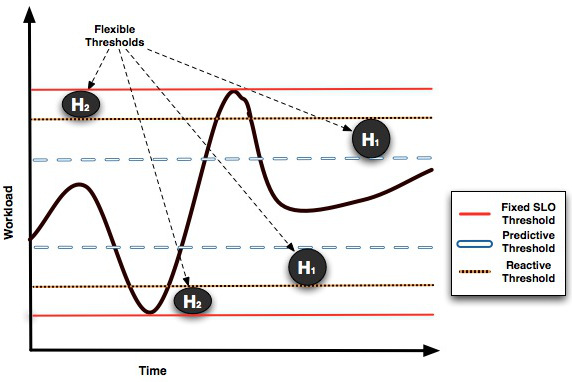
\includegraphics[width=7cm, height=5.3cm]{./images/thresholdGraphic.jpg}
\end{center}
\vspace{-5mm}
\caption{Two-level  thresholds}
\label{flexibleThresholds}
\end{figure}

%\corina{Are the terms ``constant'' and ``temporal'' alteration normally
%used in trend estimation, or are they terms that you defined yourself?
%In the second case I think we should mention something like ``we define constant alteration as...''.  
%And about flash crowds: from what I know, flash crowds last usually longer
%(in the order of hours) and we do want the system to provision extra
%resources in such a case. So if there is a spike of high workload that
%lasts for 10-15 minutes, I don't think we should call it a flash crowd --
%maybe just spike or fluctuation or something like this.}

%In order to take scaling decisiong using the feedback algorithm we now collect application-specific metrics for our measurements, evaluate the %evolution of the application workload avoiding an excessive reactive behavior, and handle threshold values that helps to predict possible SLA violations. 

%In particular, the profiling techniques appears as a solution to tackle this problems of heterogeneity.
\vspace{3mm}

%Anyway, the use of these three mechanisms must follow an order, as illustrated in Algorithm~\ref{history_prov}. Initially, the user has to specify the thresholds %ranges and give a weight to each metric. Next the flexible thresholds are defined based on Amazon recommendations and statistically-chose performance %measures~\footnote{These performance values are obtained from previous executions of the same application using similar hardware configurations.}. Once the %monitoring data is collected from the agents, the decision making process can start. Firstly, these data is analyzed to verify if it exceeds the predictive threshold %ranges (denoted by \emph{pred\_thr}), if so the probability of triggering scaling actions increases proportionally in function of the metric's weight. In order to keep %track of workload variations, this algorithm stores in a queue (denoted by \emph{q}) the most recent system performance values, and analyzed them  to estimate %the workload trend (denoted by \emph{td}).  Finally, to trigger any scaling action, a serie of conditions have to be satisfied: (i) no previous scaling actions have been %taken over the last 15min; (ii) the recent monitoring data have to exceed the predictive and reactive threshold ranges; (iii) the workload trend has to follow a %constant pattern (increasing/decreasing). 


%\subsection{Workload mix-aware provisioning}
\subsection*{Dynamic load balancing weights}

%The heterogeneity of cloud platforms, and therefore, of their VMs affect to the accuracy of the provisioning decisions. VMs with better hardware configuration can sustain higher workload intensities. In addition, the mixture of static/dynamic requests included into the workload of web applications makes more difficult to distribute these requests across multiple backend servers. Most of existing web load-balancer systems provide simple methods which do not consider the workload mix. Hence, methods such as\emph{round-robin} distributes the requests according to the servers with respect of its server weight; and the \emph{least connections} method which distributes requests to the server with the least connections. Unfortunately, these load-distribution methods are not so accurate when having a large diversity in the complexity of the requests. 

%As a solution, the workload mix-aware algorithm proposes to use a dynamic-weight load balancing method in conjunction with the feedback algorithm. By using this dynamic load-balancing mechanism, each backend server has a weight value which is dynamically adjusted based on its monitoring data, and thereby based on its own performance behavior. This mechanism allows to distribute requests across the servers taken into consideration the current workload intensity and the server throughput, which vary depending of its hardware configuration. As illustrated in Algorithm~\ref{mix_prov}, this algorithm assigns the same weight to each backend servers at the beginning of the process, and progressively adjusts their weights  (every $\sim$ 15min) depending on the monitoring data collected from each backend. By doing so, the load-balancing takes into account the complexity of the served requests and inherently the server throughput improving the distribution.

Another problem that we need to consider is the heterogeneity of cloud platforms.
Different virtual machines from the same cloud might have different performance
characteristics, even when their specifications from the cloud vendor are 
the same~\cite{ec2Performance}. This issue can be addressed through various 
load balancing techniques, like assigning weights to the backend servers or 
taking into account the current number of connections that each server 
handles. Furthermore, the performance behavior of the virtual servers may 
also fluctuate, either due to changes in the application's usage 
patterns, or due to changes related to the hosting of the virtual servers 
(e.g., VM migration).

In order to address these issues in ConPaaS we implemented a weighted 
load balancing system in which the weights of the servers are 
periodically re-adjusted automatically, based on the monitoring data.  
This method assigns the same weight to each backend server at the 
beginning of the process. The weights are then periodically
adjusted (in our experiments, every $\sim$ 15min) proportionally 
with the difference among the average response times of the servers 
during this time interval. By adding this technique to the feedback-based
algorithm, we noticed a performance improvement when running the
benchmarks.

%%%%%%%%%%%%%%%%%%%%%%%%%%
\begin{comment}
\begin{algorithm}
{\scriptsize
\SetAlgoLined
\SetInd{0mm}{2mm}
\KwData{ Pre-defined metric threshold ranges, \emph{SLO\_threshold}\\
\hspace{9mm} Define the weight of each metric, \emph{w}
}
\KwResult{Scaling decisions}
\BlankLine
Create a queue to store historical workload, \emph{q}\;
Establish flexible thresholds: \emph{pred\_thr} and \emph{reac\_thr}\; 
Initialize load-balancing weights for the backend servers\;
\BlankLine
\While{auto-scaling is ON}{
Collect monitoring data of each metric, \emph{data}\;

\uIf{ avg(data$_i$) $>=$ pred\_thr\_max$_i$}{
	Increment chances of \emph{scaling\_out} using \emph{w$_i$}, \emph{s\_out}\;
}\ElseIf{ avg(data$_i$) $<$ pred\_thr\_min$_i$}{
	Increment chances of \emph{scaling\_back} using $w_i$, \emph{s\_bck}\;
\Else{
Decrease the chances - \emph{s\_bck} or \emph{s\_out}\;
}}
\BlankLine
Add to \emph{q} the most recent workload value\;
Estimate historical workload trends (last $\sim$20min), \emph{td}\;
\hspace{3mm}	- Increasing, \emph{td} = 1 / Decreasing, \emph{td} = 0\;		
\BlankLine
\If{ no recent scaling operation}{
\uIf{ avg(data$_i$) $>=$ reac\_thr\_max$_i$ \textbf{and}  $td$ = 1 \textbf{and} \emph{s\_out} $>=$ \emph{s\_bck}}{
	ADD resources\;
}
\ElseIf{ avg(data$_i$) $<$ reac\_thr\_min$_i$ \textbf{and} \emph{td} = 0 \textbf{and} s\_out $<$ s\_bck }{
	REMOVE resources\;
}
Reset \emph{s\_bck} and\emph{s\_out}\;
}\Else{ Sleep during 5 minutes\;}
\BlankLine
Adjust load-balancing weights based on the workload ($\sim$15min)\;
}
}
\caption{Dynamic load-balancing weights}
\label{mix_prov}
\end{algorithm}
\end{comment}

%%%%%%%%%%%%%%%%%%%%%%%%%%%%%%%%%%

%\fixme{unlike in some synthetic benchmarks, in Wikipedia there are large variations
%in the complexity of the articles; so the PHP processing time is more difficult 
% to predict}

%\begin{figure}
%\begin{center}
%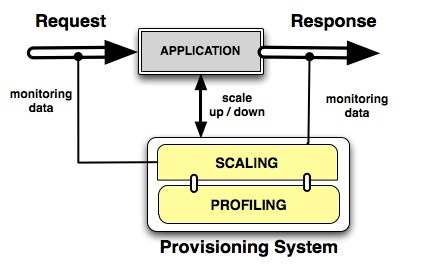
\includegraphics[width=0.4\textwidth, height=4cm]{./images/monitoringSchema.jpg}
%\end{center}
%\label{model}
%\caption{Profiling Resource Provisioning}
%\end{figure}
